% Researching sources: the stand-in for the subject librarian's hour in Week 8,
% built to be run on its own if the librarian cannot come.
% Shared preamble for the write-on class slides.
%
% Every deck is designed to be projected and annotated live on a tablet:
% whatever takes time to draw is pre-drawn, and whatever the class produces is
% left blank. Compile a deck with `pdflatex main.tex` from its own directory,
% or run `uv run python build.py` from the repository root to build them all.
% The build also compiles each deck a second time with the answers written in,
% and renders those pages as the images the facilitator notes show.
\documentclass[10pt]{article}

\usepackage[papersize={25.6cm,14.4cm}, margin=1.1cm, bottom=1.5cm,
            footskip=0.75cm]{geometry}
\usepackage[T1]{fontenc}
\usepackage[default]{sourcesanspro}
\usepackage[scaled=0.92]{sourcecodepro}
\usepackage{newtxsf}
\usepackage{tikz}
\usepackage{amsmath}
\usepackage{parskip}
\usepackage{fancyhdr}
\usetikzlibrary{arrows.meta, positioning, calc}

\setlength{\parindent}{0pt}

% Catppuccin Latte, the palette the course site uses in its light theme, so a
% deck on the projector looks like the pages the students read.
\definecolor{inkbg}{HTML}{EFF1F5}      % base
\definecolor{inksurface}{HTML}{E6E9EF} % mantle
\definecolor{inkfaint}{HTML}{CCD0DA}   % surface2, for rules and empty boxes
\definecolor{inktext}{HTML}{4C4F69}    % text
\definecolor{inkgrey}{HTML}{8C8FA1}    % overlay1, for anything secondary
\definecolor{inkblue}{HTML}{7287FD}    % lavender, the primary accent
\definecolor{inkteal}{HTML}{179299}    % teal
\definecolor{inkred}{HTML}{FE640B}     % peach, for whatever wants attention
\definecolor{inkmauve}{HTML}{8839EF}   % mauve
\definecolor{inkanswer}{HTML}{D20F39}  % red, for anything written by hand

\pagecolor{inkbg}
\color{inktext}

% Answer mode. A deck compiles blank, which is what we project, and compiles a
% second time with the answers written in when \answermode is defined ahead of
% this preamble. Both builds come from the one source, so a key cannot drift
% away from the deck it answers.
\newif\ifanswers
\ifdefined\answermode\answerstrue\fi

% Material that belongs to the answer build alone.
\newcommand{\onlyanswer}[1]{\ifanswers#1\fi}

% A box to write a short answer into. White against the tinted page, so it
% reads as somewhere to write rather than as part of the printed material.
\newcommand{\blank}[1][1.6]{%
  \tikz[baseline=(current bounding box.base)]{%
    \draw[inkfaint, line width=0.7pt, rounded corners=2pt, fill=white]
      (0,-0.18) rectangle (#1,0.62);}}

% The same box with its answer in it: blank on the projector, filled in the
% answer build. A box whose answer belongs to the room rather than to the
% material stays a plain \blank and is empty in both builds.
\newcommand{\answerblank}[2][1.6]{%
  \tikz[baseline=(current bounding box.base)]{%
    \draw[inkfaint, line width=0.7pt, rounded corners=2pt, fill=white]
      (0,-0.18) rectangle (#1,0.62);
    \onlyanswer{%
      \node[text=inkanswer, font=\small, inner sep=1pt, align=center,
            anchor=center, draw=none, fill=none, text width=,
            minimum width=0pt, minimum height=0pt]
        at (#1/2,0.22) {#2};}}}

% The ruled area itself, drawn inside a picture the caller owns.
\newcommand{\workspacebox}[2]{%
  \draw[inkfaint, line width=0.7pt, rounded corners=3pt, fill=white]
    (0,0) rectangle (#1,#2);
  \foreach \gx in {0.5,1.0,...,#1}{%
    \foreach \gy in {0.5,1.0,...,#2}{%
      \fill[inkfaint] (\gx,\gy) circle (0.5pt);}}}

% A ruled area to work in. Faint dots keep handwriting level on a tablet.
\newcommand{\workspace}[2]{%
  \begin{tikzpicture}\workspacebox{#1}{#2}\end{tikzpicture}}

% A ruled area with the answer in it: empty on the projector, written in for
% the answer build.
\newcommand{\answerspace}[3]{%
  \begin{tikzpicture}
    \workspacebox{#1}{#2}
    \onlyanswer{%
      \node[text=inkanswer, anchor=north west, align=left, font=\large,
            text width=\dimexpr#1cm-0.9cm\relax]
        at (0.45,#2-0.35) {#3};}
  \end{tikzpicture}}

% A panel for material that is printed rather than written on.
\newcommand{\panel}[2]{%
  \begin{tikzpicture}
    \draw[inkfaint, line width=0.7pt, rounded corners=3pt, fill=inksurface]
      (0,0) rectangle (#1,#2);
  \end{tikzpicture}}

% A labelled card of printed material. #2 and #3 are widths in cm; the text
% column is the card less its padding, computed rather than guessed.
\newcommand{\cardbox}[4]{%
  \begin{tikzpicture}
    \node[draw=#1, line width=1pt, rounded corners=4pt, fill=white,
          minimum width=#2cm, minimum height=#3cm,
          text width=\dimexpr#2cm-0.9cm\relax,
          align=left, inner sep=0.45cm, text=inktext] {#4};
  \end{tikzpicture}}

% A card whose body is left blank for the class to fill in.
\newcommand{\cardblank}[4]{%
  \begin{tikzpicture}
    \node[draw=#1, line width=1pt, rounded corners=4pt, fill=white,
          minimum width=#2cm, minimum height=#3cm,
          text width=\dimexpr#2cm-0.9cm\relax,
          align=left, inner sep=0.45cm, text=inktext, anchor=north west]
      at (0,0) {#4};
  \end{tikzpicture}}

% Running header: the deck name on the left, the page's own step on the right.
% Each deck sets its name once with \deckname.
\newcommand{\deck}{}
\newcommand{\deckname}[1]{\renewcommand{\deck}{#1}}
\newcommand{\slidehead}[1]{%
  {\small\color{inkgrey}%
   \tikz[baseline=-0.5ex]{\fill[inkblue, rounded corners=1pt]
     (0,0) rectangle (0.22,0.22);}\;\deck
   \hfill \color{inkblue}\bfseries #1}\par
  {\color{inkblue}\rule{\linewidth}{1pt}}\par\vspace{0.35em}}

\pagestyle{fancy}
\fancyhf{}
\renewcommand{\headrulewidth}{0pt}
\fancyfoot[R]{\small\color{inkgrey}\thepage}

% A pointer into the notes at the foot of a slide, so that the hour reads as a
% way through the reading rather than a detour from it. The first argument
% names the notes and the second the section. Each page sets its own, which is
% read when the page is shipped out, so a page with nothing to point at calls
% \nonotes.
\newcommand{\notesline}{}
\newcommand{\notesref}[2]{\gdef\notesline{%
  \tikz[baseline=-0.5ex]{\fill[inkteal, rounded corners=1pt]
    (0,0) rectangle (0.24,0.24);}\;\textbf{#1}\; #2}}
\newcommand{\nonotes}{\gdef\notesline{}}
\fancyfoot[L]{\small\color{inkteal}\notesline}

% Deck title pages, which carry no header and no page number.
\newcommand{\titleslide}[3]{%
  \thispagestyle{empty}%
  \begin{center}
    \vspace*{\fill}
    {\Huge\bfseries\color{inkblue} #1}\\[0.7em]
    {\LARGE\color{inkgrey} #2}\\[2.4em]
    #3
    \vspace*{\fill}
  \end{center}}

% One step of the plan on a title page.
\newcommand{\stepbox}[3]{%
  \node[draw=inkblue, line width=0.9pt, rounded corners=4pt, fill=white,
        minimum width=6cm, minimum height=1.7cm, align=center,
        text=inktext] (#1) at (#2,0) {#3};}

% Prompt to the room: a question the class answers, not something I read out.
\newcommand{\ask}[1]{%
  {\large\color{inkblue}\bfseries #1}\par\vspace{0.5em}}

% A block of code. #1 is the width in cm, #2 the lines, separated by \\ and
% indented with \idt. Set against white so it reads as a listing rather than
% as prose.
\newcommand{\idt}{\hspace*{1.4em}}
\newcommand{\codebox}[2]{%
  \begin{tikzpicture}
    \node[draw=inkfaint, line width=0.7pt, rounded corners=3pt, fill=white,
          minimum width=#1cm, text width=\dimexpr#1cm-1.0cm\relax,
          align=left, inner sep=0.5cm, text=inktext,
          font=\ttfamily\large] {#2};
  \end{tikzpicture}}

% A line of code that is wrong, for the slides that ask the class what breaks.
\newcommand{\wrong}[1]{\textcolor{inkred}{#1}}

% A backslash inside a listing, for the slides that show LaTeX source.
\newcommand{\bs}{\textbackslash}


\deckname{Researching sources}

\begin{document}

\titleslide{Researching sources}{Week 8. The 20\% nobody prepares for.}{%
    
\begin{tikzpicture}[font=\small]
      \stepbox{s0}{0.0}{\textbf{Find}\\[0.25em] What already exists.}
      \stepbox{s1}{6.9}{\textbf{Judge}\\[0.25em] Is it worth citing?}
      \stepbox{s2}{13.8}{\textbf{Cite}\\[0.25em] In the prose, not a list.}
      \draw[-{Stealth[length=2.5mm]}, inkfaint, line width=1.2pt] (s0) -- (s1);
      \draw[-{Stealth[length=2.5mm]}, inkfaint, line width=1.2pt] (s1) -- (s2);
    \end{tikzpicture}}

\newpage
\slidehead{Research is 20\% of the project mark}

\vspace{1.1cm}

{\LARGE
\textbf{\color{inkblue}State of the field.}\quad How does your library
compare with the tools that already exist?

\vspace{1.3em}

\textbf{\color{inkteal}References.}\quad Is everything that should be
cited actually cited, in the text, properly?}

\vspace{1.6cm}

\begin{center}
{\large\color{inkgrey} This is the component groups lose most marks on,
and the cheapest one to fix.}
\end{center}

\newpage
\slidehead{Four things you will need to cite}

\vspace{0.9cm}

\begin{center}
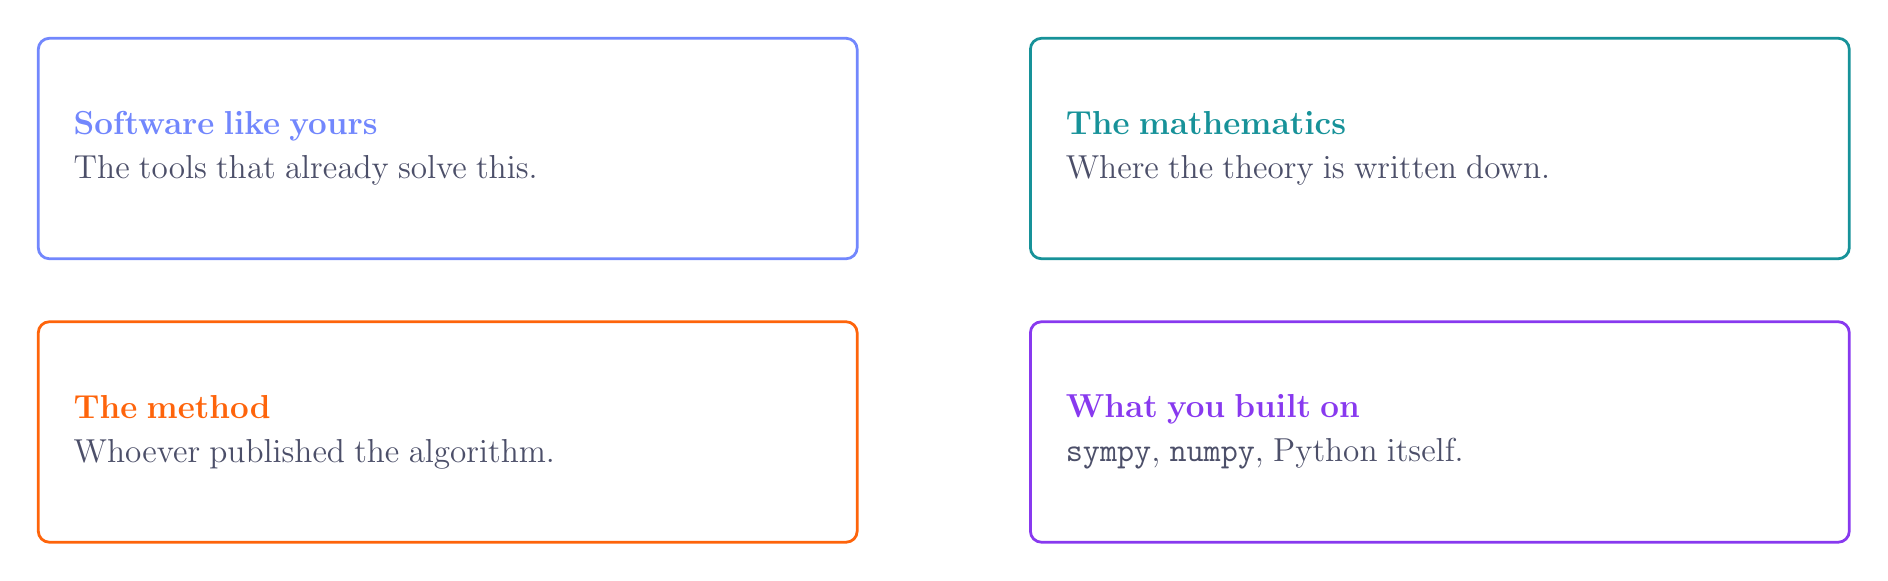
\begin{tikzpicture}
  \node at (0,0) {\cardbox{inkblue}{10.4}{2.8}{%
    {\large\bfseries\color{inkblue} Software like yours}\\[0.4em]
    {\large The tools that already solve this.}}};
  \node at (12.6,0) {\cardbox{inkteal}{10.4}{2.8}{%
    {\large\bfseries\color{inkteal} The mathematics}\\[0.4em]
    {\large Where the theory is written down.}}};
  \node at (0,-3.6) {\cardbox{inkred}{10.4}{2.8}{%
    {\large\bfseries\color{inkred} The method}\\[0.4em]
    {\large Whoever published the algorithm.}}};
  \node at (12.6,-3.6) {\cardbox{inkmauve}{10.4}{2.8}{%
    {\large\bfseries\color{inkmauve} What you built on}\\[0.4em]
    {\large \texttt{sympy}, \texttt{numpy}, Python itself.}}};
\end{tikzpicture}
\end{center}

\vspace{0.8cm}

\ask{Which of the four does your group already have?}

\newpage
\slidehead{Where to look}

\vspace{1.0cm}

{\LARGE
\textbf{\color{inkblue}The library.}\quad The discovery service, for
textbooks and journals you can actually open.

\vspace{1.0em}

\textbf{\color{inkteal}Google Scholar and arXiv.}\quad For papers, and
for the citation count that tells you who is read.

\vspace{1.0em}

\textbf{\color{inkred}PyPI and the docs.}\quad For the software. The
project's own documentation is a citable source.

\vspace{1.0em}

\textbf{\color{inkmauve}JOSS.}\quad Papers about libraries exactly like
yours, and the criteria yours is marked against.}

\vspace{1.2cm}

{\small\color{inkgrey} A web search is where you start, not what you
cite. Follow it to the thing itself.}

\newpage
\slidehead{Your state of the field, in one question}

\vspace{0.5cm}

\ask{Name three tools that already do something like what your library
does. For each one, say what yours does differently.}

\vspace{0.3em}

\begin{center}
\workspace{22}{7.0}
\end{center}

\vspace{0.2cm}

{\small\color{inkgrey} `There is nothing else like it' is almost never
true, and it is the answer that scores worst.}

\newpage
\slidehead{Is it worth citing?}

\vspace{0.9cm}

\begin{center}

\begin{tikzpicture}
  \node at (0,0) {\cardblank{inkblue}{5.0}{4.6}{%
    {\large\bfseries\color{inkblue} Who wrote it?}}};
  \node at (5.85,0) {\cardblank{inkteal}{5.0}{4.6}{%
    {\large\bfseries\color{inkteal} Still current?}}};
  \node at (11.7,0) {\cardblank{inkred}{5.0}{4.6}{%
    {\large\bfseries\color{inkred} Who else cites it?}}};
  \node at (17.55,0) {\cardblank{inkmauve}{5.0}{4.6}{%
    {\large\bfseries\color{inkmauve} Can you check it?}}};
\end{tikzpicture}
\end{center}

\vspace{1.0cm}

\ask{Four questions, four answers. What does a good source look like on
each one?}

\vspace{0.3cm}

{\small\color{inkgrey} The last one matters most. If you cannot verify
the claim yourself, you are repeating it, not citing it.}

\newpage
\slidehead{Same claim, three places}

\vspace{0.7cm}

\begin{center}

\begin{tikzpicture}
  \node at (0,0) {\cardbox{inkred}{6.8}{2.6}{%
    {\large\bfseries\color{inkred} A forum answer}\\[0.3em]
    {\large Anonymous. Undated.}}};
  \node at (8.1,0) {\cardbox{inkteal}{6.8}{2.6}{%
    {\large\bfseries\color{inkteal} The docs}\\[0.3em]
    {\large Written by its authors.}}};
  \node at (16.2,0) {\cardbox{inkblue}{6.8}{2.6}{%
    {\large\bfseries\color{inkblue} A textbook}\\[0.3em]
    {\large Edited. Peer reviewed.}}};
\end{tikzpicture}
\end{center}

\vspace{0.9cm}

\ask{All three tell you the same thing. Which do you cite, and for what?}

\vspace{0.3em}

\begin{center}
\workspace{22}{3.8}
\end{center}

\newpage
\slidehead{What a reference actually is}

\vspace{0.4cm}

\begin{minipage}[t]{0.56\linewidth}
\vspace{0pt}
\codebox{12.6}{@article\{meurer2017,\\
\idt author = \{Meurer, Aaron and others\},\\
\idt title = \{SymPy: symbolic computing\},\\
\idt journal = \{PeerJ Computer Science\},\\
\idt year = \{2017\},\\
\idt doi = \{10.7717/peerj-cs.103\}\\
\}}
\end{minipage}
\hfill
\begin{minipage}[t]{0.40\linewidth}
\vspace{0pt}
\ask{Nobody types this. Where does it come from?}

\workspace{9.0}{5.4}
\end{minipage}

\vspace{0.2cm}

{\small\color{inkgrey} Google Scholar's `Cite' gives you BibTeX. So does
the DOI, and so does Zotero. Paste it into
\texttt{references.bib} and never retype a reference again.}

\newpage
\slidehead{Then four commands, in order}

\vspace{1.0cm}

\begin{center}

\begin{tikzpicture}
  \foreach \lbl/\x/\n in {pdflatex/0/a, bibtex/5.6/b, pdflatex/11.2/c,
                          pdflatex/16.8/d}{%
    \node[draw=inkblue, line width=1pt, rounded corners=4pt, fill=white,
          minimum width=4.4cm, minimum height=1.8cm, font=\large\ttfamily,
          text=inkblue] (\n) at (\x,0) {\lbl};}
  \foreach \p/\q in {a/b, b/c, c/d}{%
    \draw[-{Stealth[length=2.5mm]}, inkfaint, line width=1.3pt] (\p) -- (\q);}
\end{tikzpicture}
\end{center}

\vspace{1.3cm}

\ask{Your paper says \texttt{[?]} where a citation should be. Which one
have you not run?}

\vspace{1.0cm}

{\small\color{inkgrey} Overleaf does all four for you. A local install
does not. Cross references need the second \texttt{pdflatex} too.}

\newpage
\slidehead{A reference doing work}

\vspace{1.0cm}

\begin{center}
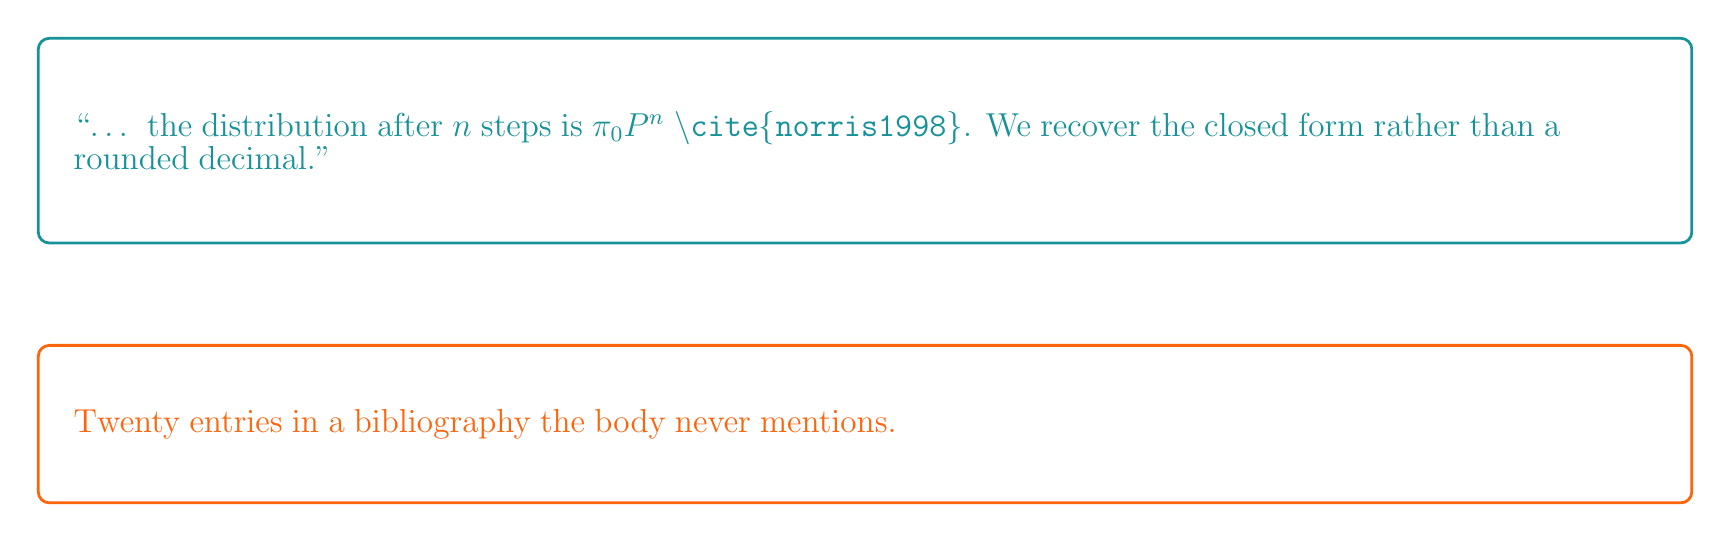
\begin{tikzpicture}
  \node at (0,0) {\cardbox{inkteal}{21}{2.6}{%
    {\large\color{inkteal} ``\ldots{} the distribution after \(n\) steps is
     \(\pi_0 P^n\)~\texttt{\bs cite\{norris1998\}}. We recover the closed
     form rather than a rounded decimal.''}}};
  \node at (0,-3.6) {\cardbox{inkred}{21}{2.0}{%
    {\large\color{inkred} Twenty entries in a bibliography the body never
     mentions.}}};
\end{tikzpicture}
\end{center}

\vspace{1.0cm}

\begin{center}
{\LARGE A paper that argues with four references beats one that lists
twenty.}
\end{center}

\newpage
\slidehead{Write the paragraph now}

\vspace{0.5cm}

\ask{Three or four sentences. What exists, what it does, what yours does
that it does not, and why that is worth doing.}

\vspace{0.3em}

\begin{center}
\workspace{22}{7.2}
\end{center}

\vspace{0.2cm}

{\small\color{inkgrey} This paragraph goes in your introduction. Writing
it now means the rest of the paper has something to point at.}

\newpage
\slidehead{Before you leave}

\vspace{0.8cm}

\begin{center}
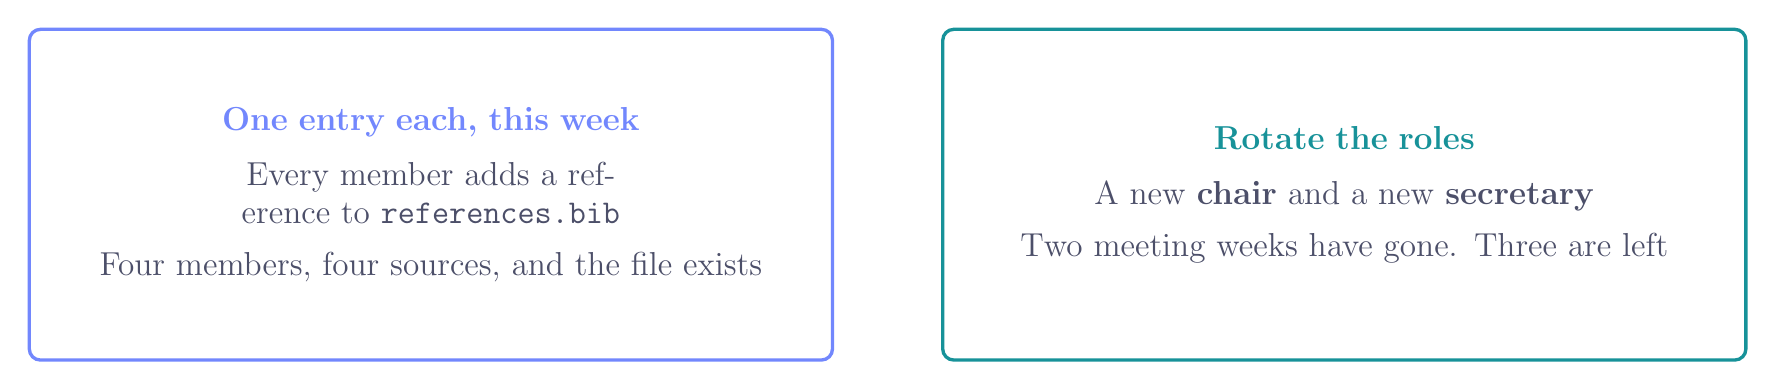
\begin{tikzpicture}
  \node[draw=inkblue, line width=1.2pt, rounded corners=4pt, fill=white,
        minimum width=10.2cm, minimum height=4.2cm, text width=9.2cm,
        align=center, inner sep=0.4cm, text=inktext, font=\large] at (0,0) {%
    \textbf{\color{inkblue} One entry each, this week}\\[0.5em]
    Every member adds a reference to
    \texttt{references.bib}\\[0.4em]
    Four members, four sources, and the file exists};
  \node[draw=inkteal, line width=1.2pt, rounded corners=4pt, fill=white,
        minimum width=10.2cm, minimum height=4.2cm, text width=9.2cm,
        align=center, inner sep=0.4cm, text=inktext, font=\large]
    at (11.6,0) {%
    \textbf{\color{inkteal} Rotate the roles}\\[0.5em]
    A new \textbf{chair} and a new \textbf{secretary}\\[0.4em]
    Two meeting weeks have gone. Three are left};
\end{tikzpicture}
\end{center}

\vspace{0.9cm}

\begin{center}

\begin{tikzpicture}
  \node[draw=inkred, line width=1.4pt, rounded corners=4pt, fill=white,
        minimum width=21.8cm, minimum height=2.2cm, text width=20.6cm,
        align=center, inner sep=0.35cm, text=inktext, font=\large] {%
    \textbf{\color{inkred} Meet this week. Bring the Week 9 minutes to the
    next session.}\quad The fourth of the five that \(I\) is counted from.};
\end{tikzpicture}
\end{center}

\end{document}
